\section{Introduction}
\label{sec:introduction}

\begin{figure*}[t]
    \centering
    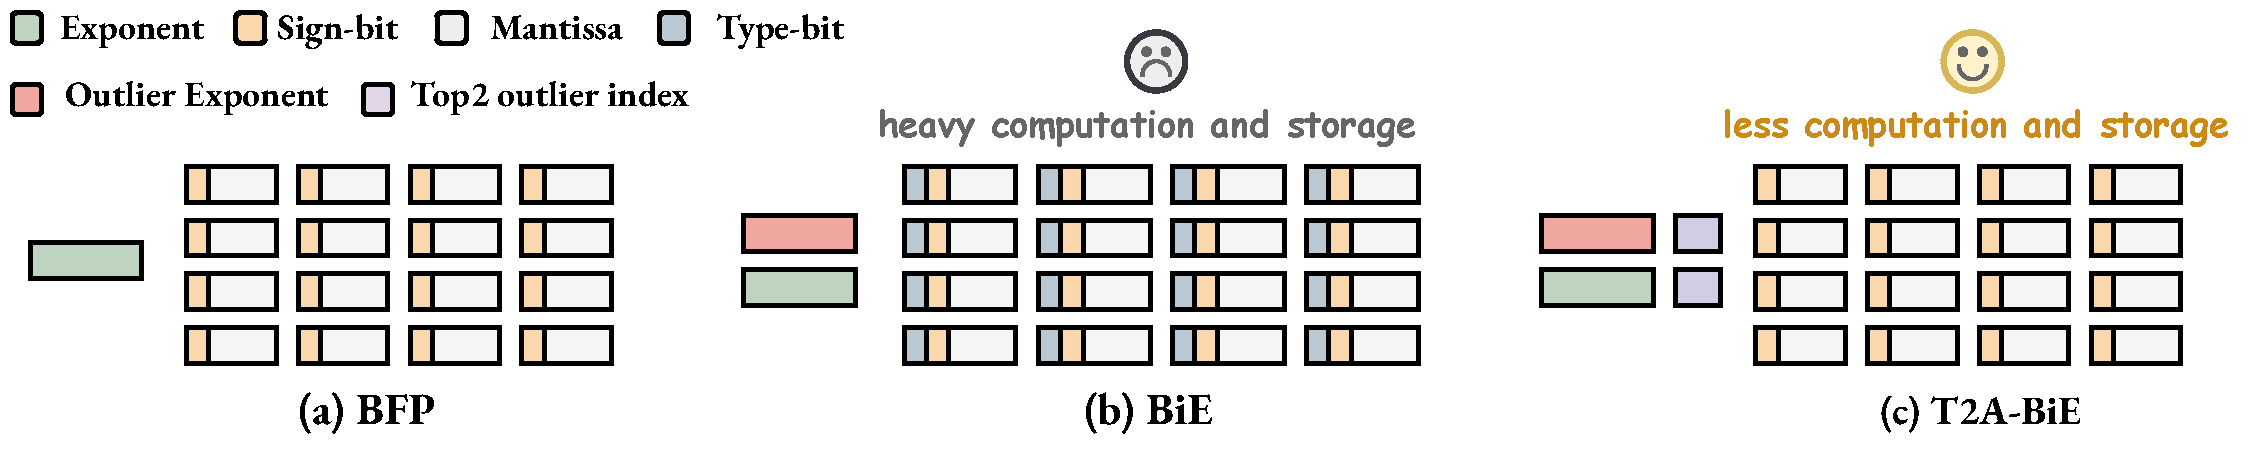
\includegraphics[width=0.95\textwidth]{figures/data-format.pdf}
    \caption{Block-level data formats. (a) Conventional BFP with one shared exponent per block. (b) Bi-exponent BFP (BiE), which adds an outlier exponent and spends a type bit on every element. (c) The proposed Top-2 Activation-only Bi-Exponent BFP (T2A-BiE), which keeps both exponents but replaces the per-element type bits with two outlier indices, so the storage and MAC overhead is lower than that of BiE; weights remain single-exponent BFP as in (a).}
    \label{fig:data_format}

    \vspace{4pt}
    \begin{minipage}[t]{0.48\textwidth}
        \centering
        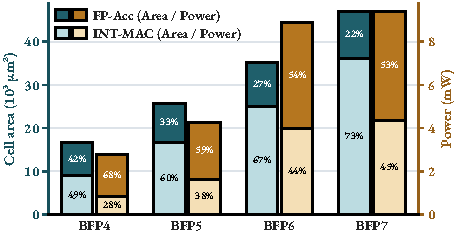
\includegraphics[width=\linewidth]{figures/baseline_bfp_pe_component_power_area.pdf}
        \caption{Component-level power and area of a synthesized baseline BFP-PE (TSMC 90\,nm, 100\,MHz). Power is measured under LLaMA2-7B's real activation distribution.}
        \label{fig:bfp_pe_ppa}
    \end{minipage}%
    \hfill
    \begin{minipage}[t]{0.48\textwidth}
        \centering
        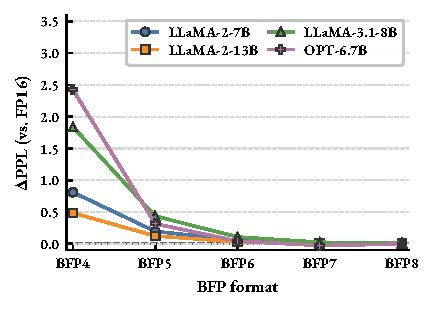
\includegraphics[width=\linewidth]{figures/vanilla_bfp_delta_ppl_g16.pdf}
        \caption{WikiText-2 $\Delta$PPL of vanilla BFP versus FP16 as the mantissa width decreases (group size 16).}
        \label{fig:vanilla_bfp_delta_ppl}
    \end{minipage}
\end{figure*}

Low-precision quantization is essential for deploying large language models (LLMs) under tight memory and energy budgets.
Power is a first-class constraint in this context: industrial inference accelerators are designed around thermal design power because TDP tracks total cost of ownership, whereas area-based metrics such as performance per square millimeter can look favorable even when energy cost rises~\cite{tpuv4i2021}.
Block Floating Point (BFP) offers a compelling accuracy--cost tradeoff by partitioning tensors into fixed-size blocks, each with a shared exponent, and storing only low-bit mantissas~\cite{msfp2020,fast2022}.
Recent BFP accelerators exploit this structure to perform intra-block multiply--accumulate (MAC) operations with fixed-point arithmetic, but inter-block partial sums whose shared exponents differ must still be merged in a floating-point accumulator (FP-Acc)~\cite{bucketgetter2023,winacc2025,smartblock2025,mgs2025}.

Two coupled bottlenecks limit the efficiency of BFP-based LLM inference.
First, the FP-Acc dominates processing-element (PE) cost.
As the mantissa width shrinks, the fixed-point multipliers and adder tree become smaller while the FP-Acc stays the same size, so its share of total PE power and area grows (Fig.~\ref{fig:bfp_pe_ppa}).
Second, activation outliers---values whose magnitude far exceeds that of co-located elements---compress the effective mantissa of normal values and widen the exponent spread of partial sums, increasing the frequency at which the FP-Acc must be invoked~\cite{bie2024,ees2025,oiso2026,bbal2025,harmonia2026}.
These two bottlenecks reinforce each other: the outliers that degrade quantization accuracy also inflate FP-Acc activity, so addressing them jointly is more effective than tackling either in isolation.

This paper develops a hardware-friendly co-design that targets both bottlenecks.
Our contributions are:
\begin{itemize}
    \item \textbf{Dynamic Exponent-Window Accumulation (DEWA):} a lightweight integer accumulator that retains partial sums within a sliding exponent window and forwards only out-of-window events to the FP-Acc, substantially reducing its utilization.
    \item \textbf{Activation-only bi-exponent encoding with Top-2 selection (T2A-BiE):} weights remain in single-exponent BFP while each activation block carries a second exponent for at most two outlier lanes, reducing storage and MAC control overhead relative to full bi-exponent encoding~\cite{bie2024,oiso2026}.
    \item \textbf{End-to-end evaluation:} we validate the proposed W-BFP4 / T2A-BiE4 design point on LLaMA2-7B, LLaMA-3.1-8B, and OPT-6.7B, demonstrating that the combined scheme preserves model accuracy while delivering a PE that is both smaller and more energy-efficient than a conventional BFP baseline and a recent BFP accelerator.
\end{itemize}

The remainder of this paper reviews BFP deployment challenges (Section~\ref{sec:background}), presents DEWA, Top-2 selection, and their combination (Section~\ref{sec:design}), describes the Top-2 index encoding and the DEW-based PE datapath (Section~\ref{sec:architecture}), reports experimental results (Section~\ref{sec:evaluation}), and concludes (Section~\ref{sec:conclusion}).
